


\documentclass[english,11pt]{beamer}

\DeclareMathOperator{\Cov}{Cov}
\DeclareMathOperator{\Var}{Var}
\DeclareMathOperator{\E}{\mathbb{E}}
\DeclareMathOperator{\Proba}{\mathbb{P}}

\newcommand{\Covb}[2]{\ensuremath{\Cov\!\left[#1,#2\right]}}
\newcommand{\Eb}[1]{\ensuremath{\E\!\left[#1\right]}}
\newcommand{\Pb}[1]{\ensuremath{\Proba\!\left[#1\right]}}
\newcommand{\Varb}[1]{\ensuremath{\Var\!\left[#1\right]}}

% norm
\newcommand{\norm}[1]{\| #1 \|}

\newcommand{\indep}{\rotatebox[origin=c]{90}{$\models$}}





\usepackage{mathptmx,amsmath,amssymb,graphicx,bibentry,bbm,babel,ragged2e}

\makeatletter

\newcommand{\noun}[1]{\textsc{#1}}
\newcommand{\jitem}[1]{\item \begin{justify} #1 \end{justify} \vfill{}}
\newcommand{\sframe}[2]{\frame{\frametitle{#1} #2}}

\newenvironment{centercolumns}{\begin{columns}[c]}{\end{columns}}
%\newenvironment{jitem}{\begin{justify}\begin{itemize}}{\end{itemize}\end{justify}}

\usetheme{Warsaw}
\setbeamertemplate{footline}[text line]{}
\setbeamertemplate{headline}{}
\setbeamercolor{structure}{fg=purple!50!blue, bg=purple!50!blue}

\setbeamersize{text margin left=15pt,text margin right=15pt}

\setbeamercovered{transparent}


\@ifundefined{showcaptionsetup}{}{%
 \PassOptionsToPackage{caption=false}{subfig}}
\usepackage{subfig}

\usepackage[utf8]{inputenc}
\usepackage[T1]{fontenc}

\usepackage{multirow}

\usepackage{mdframed}


\AtBeginSection[]
{
  \begin{frame}
  \frametitle{Coupling heterogeneous urban models}
  \tableofcontents[currentsection]
  \end{frame}
}

\makeatother

\begin{document}



\title{Coupling heterogeneous urban models}

\author{J.~Raimbault$^{1,2,3,4, \ast}$ and M.~Batty$^{2}$\\
$\ast$\texttt{juste.raimbault@ign.fr}
}


\institute{$^{1}$LASTIG, Univ Gustave Eiffel, IGN-ENSG\\
$^{2}$CASA, UCL\\
$^{3}$UPS CNRS 3611 ISC-PIF\\
$^{4}$UMR CNRS 8504 G{\'e}ographie-cit{\'e}s
}


\date{\textbf{Applied Urban Modelling 2022 Symposium}\\
Session 11: Advances in model integration\\
30/06/2020
}




%The integration of multiple dimensions of urban systems is essential for their  sustainable planning and management. As decision‐making tools, simulation  models are in that context a useful medium to link together these various  aspects. The coupling of heterogeneous urban models, in terms of scale,  ontology, data, and implementation among others, is therefore an important  methodological hurdle to be dealt with. In this contribution, we summarise some  recent use of scientific workflow engines to build modular urban models. In  particular, the OpenMOLE workflow engine enables seamless modle embedding ‐ whatever the implementation ‐ and provides a scripting language  which is used to couple such heterogeneous models and implement the  intermediate tasks, resulting in some sort of meta‐model in the workflow  engine. We illustrate this by coupling the QUANT spatial interaction model with  the SPENSER microsimulation model, for the case of the planned Cambridge‐ Oxford railway corridor.

%This coupling allows anticipating the infrastructure impacts within the projected  demographic context. The second illustration we develop is the coupling of the  Matsim transport model with QUANT and SPENSER to build a four‐step multimodal transport model generic to any UK functional area. We  show the advantage of using this approach by applying model validation methods provided by the OpenMOLE platform: first by running a Global Sensitivity Analysis to model parameters, and second by applying a genetic calibration algorithm to adjust mode shares to observed commuting flows.

% - insist on openmole, demo?
% - mention Dafni? (openmole integration?) - no methods - docker only
% - position % Harmony project - framework ; other presented in the session?
% - crucial points: reprod, testable/ validable workflow, open : // soduco; repository, traceability etc.


\frame{\maketitle}


\section{Integration of urban models}




\sframe{Modeling urban complexity}{


\textit{Large scale urban models are intrinsically flawed and do not reach their goals of long-term application to planning}: \textbf{Requiem for large scale models in 1973} \cite{lee1973requiem}

\bigskip


\textit{Urban analytics and Smart Cities approaches may follow the same path if they ignore the past and the complexity of cities} \cite{batty2014can}


\bigskip


To foster relevance of large urban models:

\begin{itemize}
	\item Transparency on data and implementation, reproducibility
	\item Validation of models and sub-models: from small simple models well validated to larger integrated models
\end{itemize}

\medskip

$\rightarrow$ Open, reproducible urban models can be shared, coupled into modular integrated models, tested and validated \cite{banos2013pour}

}


\sframe{Proposed research framework}{

\justify

\textbf{Sustainable urban systems: } (i) multiple contradictory objectives; (ii) implemented by stakeholders at different scales, within various information and power contexts; (iii) adaptive on multiple time scales.


\bigskip

\textbf{Models are essential tools to } (i) capture complexity; (ii) construct integrated perspectives; (iii) link data, empirical stylised facts and decision-making.

\bigskip


$\rightarrow$ \textbf{Integrated models} to simulate multiple dimensions of \textbf{urban systems} towards decision-making in the context of \textbf{sustainable transitions}.

\bigskip

\begin{itemize}
	\item Horizontal integration (model coupling and interdisciplinarity)
	\item Vertical integration (multi-scale models)
	\item Model exploration and validation methods
\end{itemize}


}



\sframe{Horizontal integration: interdisciplinarity}{

\textit{Literature mapping and systematic review tools to enhance integration}

\medskip

\begin{center}
	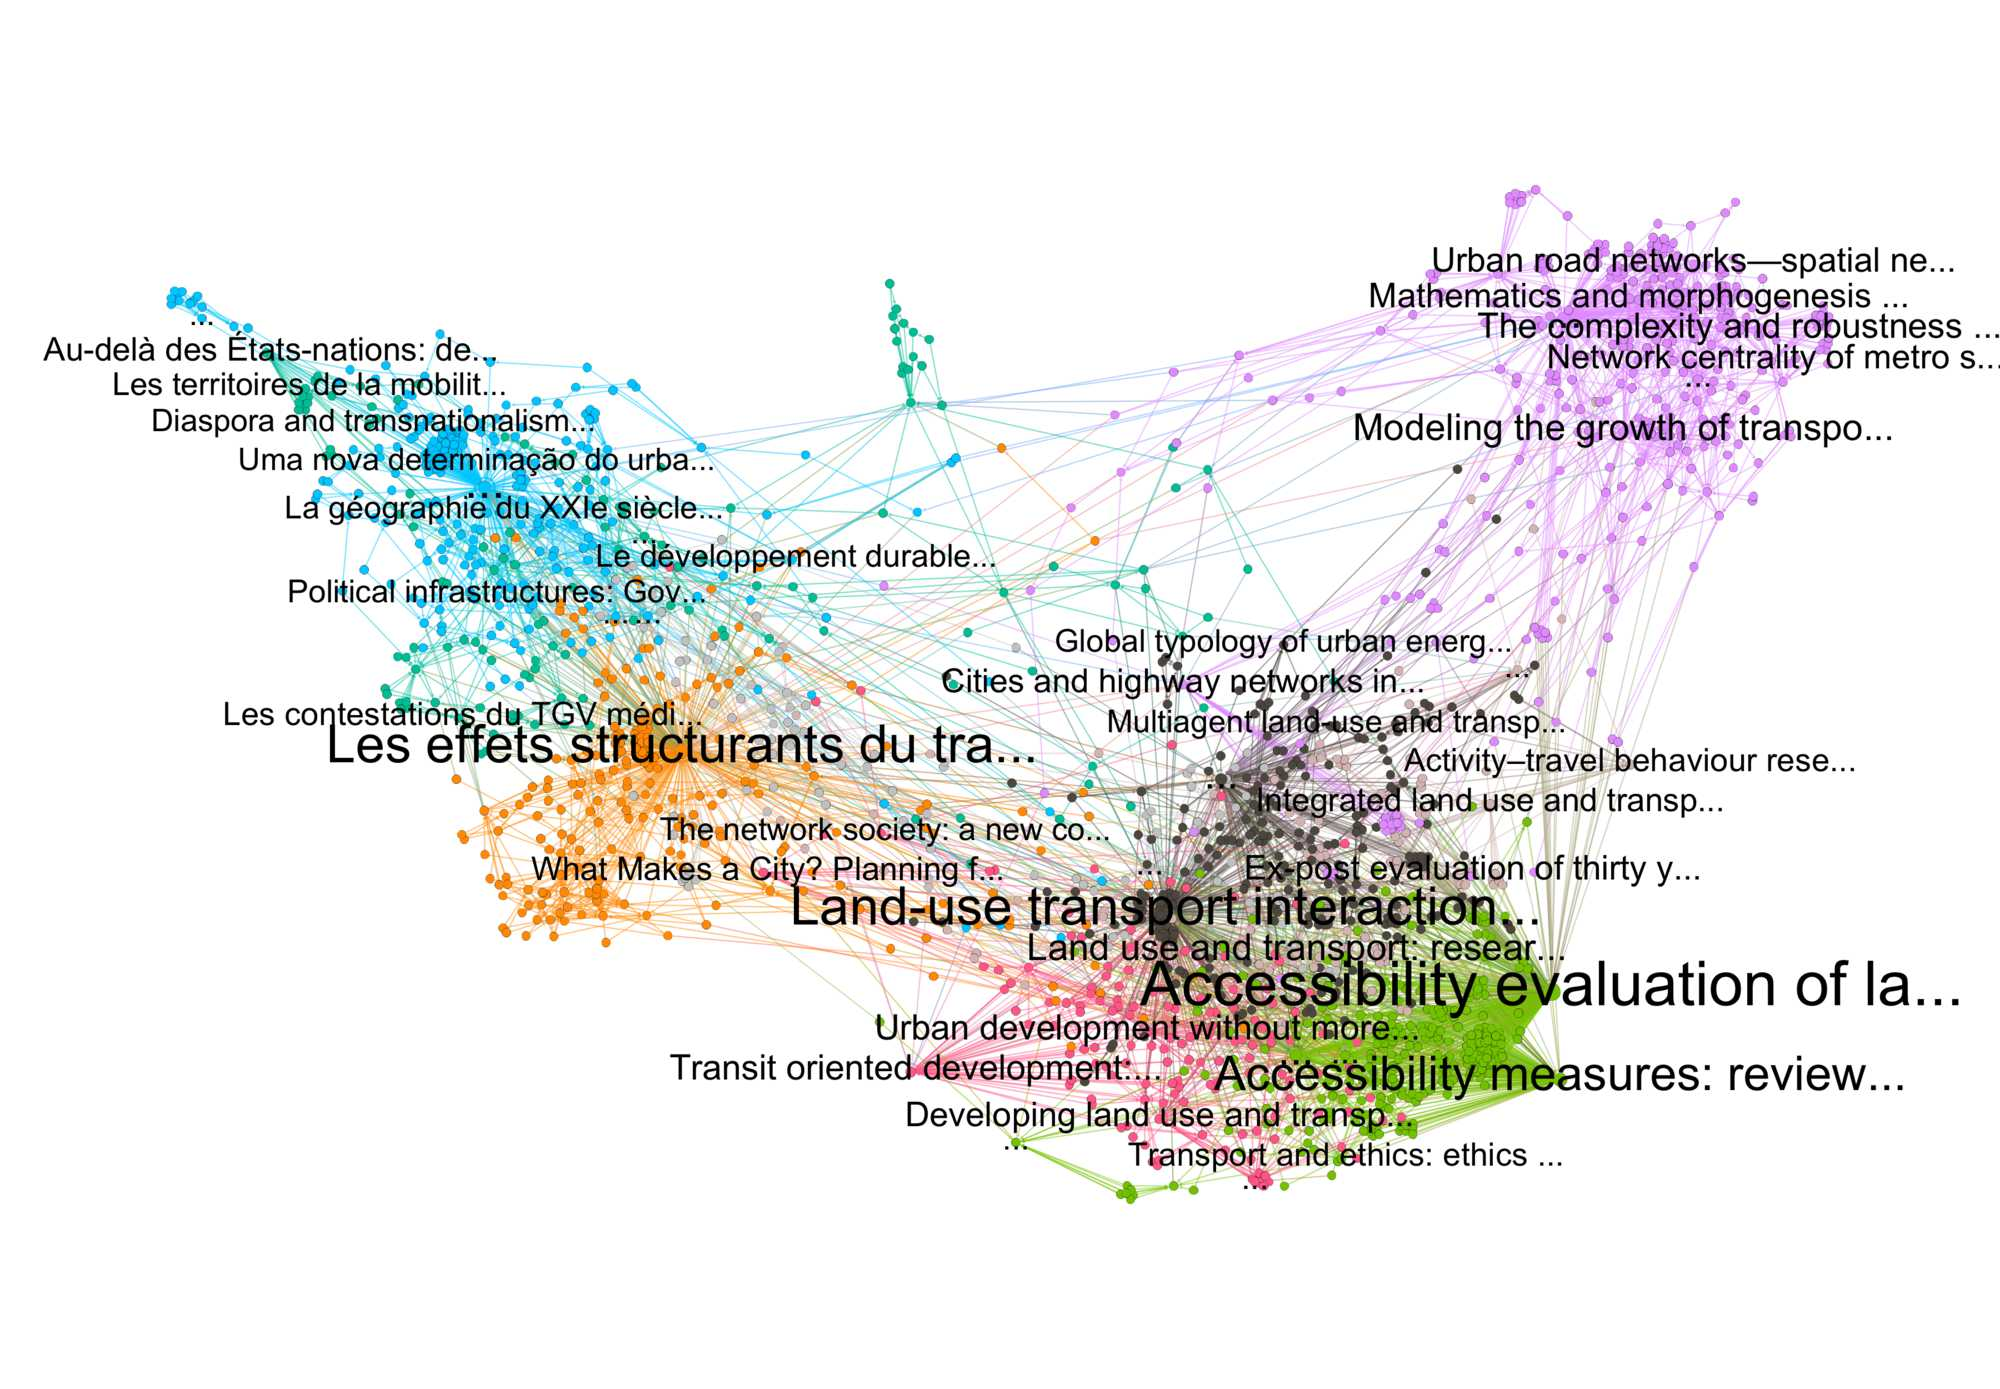
\includegraphics[width=0.9\textwidth,trim={0 2cm 0 2cm},clip]{figures/2-2-2-fig-quantepistemo-citnw.jpg}	
\end{center}

\medskip

\tiny

\vspace{-1cm}

Raimbault, J. (2019). Exploration of an interdisciplinary scientific landscape. Scientometrics, 119(2), 617-641.

\nocite{raimbault2019exploration}

}



\sframe{Horizontal integration: multi-modeling and benchmarks}{


\begin{center}
	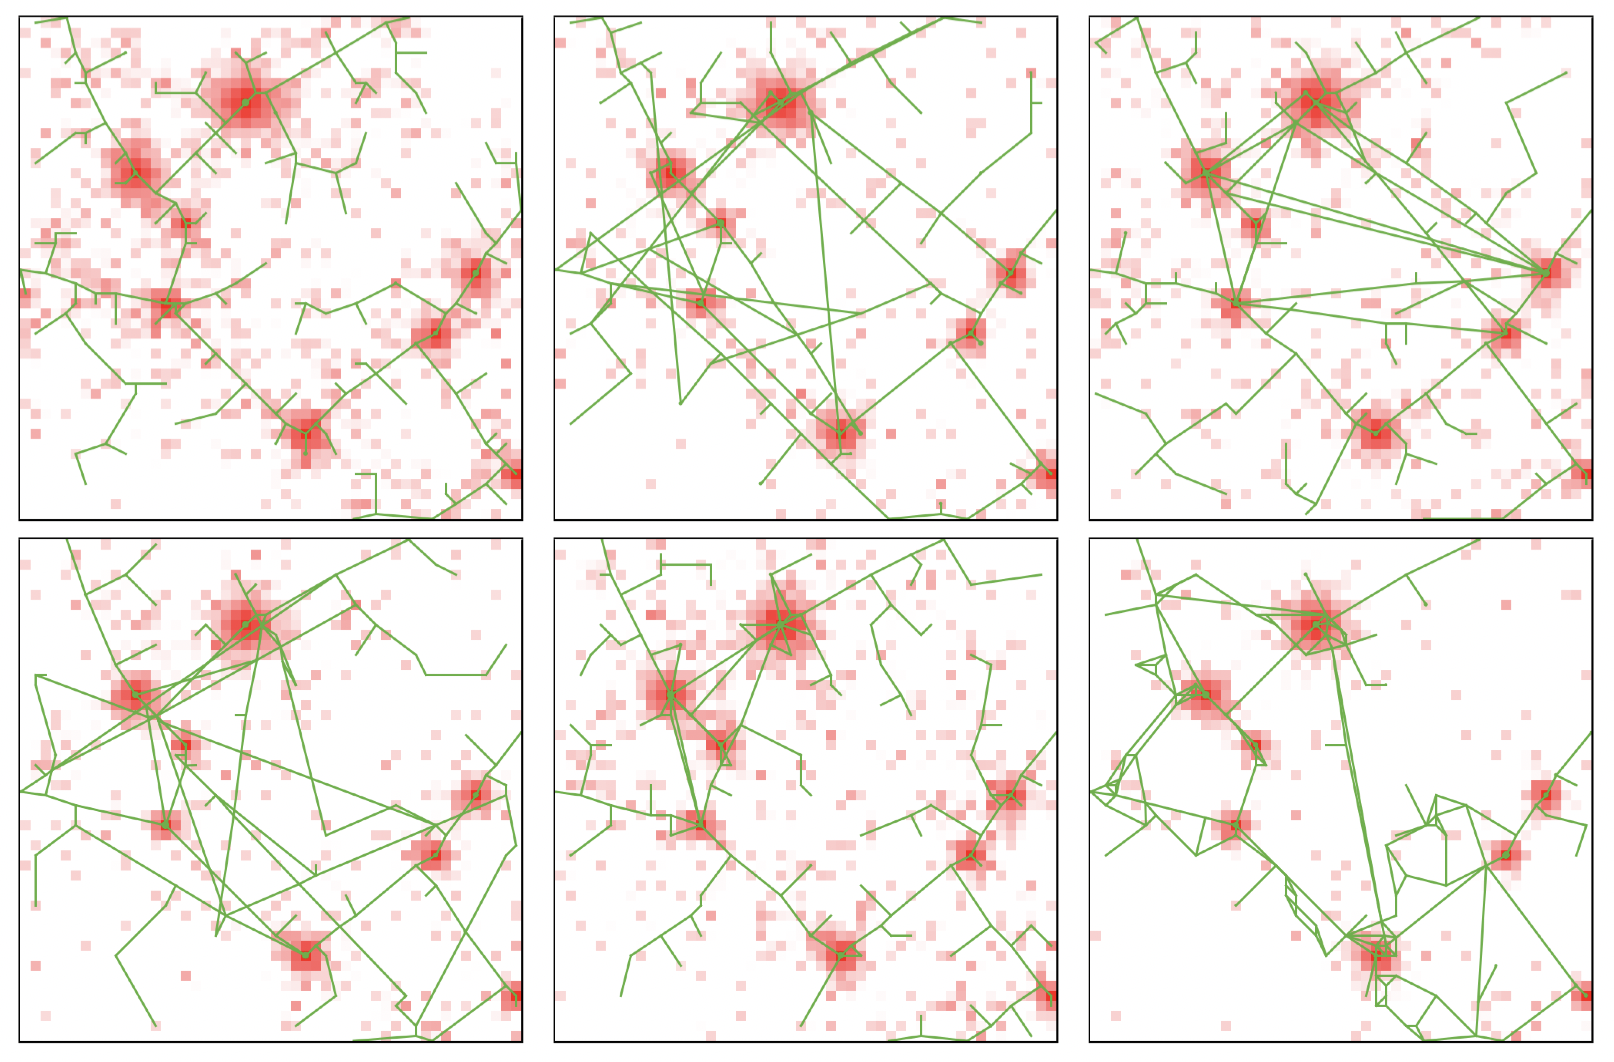
\includegraphics[width=0.56\linewidth]{figures/meso_multimodeling.png}\hspace{0.5cm}
	
\includegraphics[width=0.36\linewidth]{figures/mesobench_Fig3.png}
\end{center}

\medskip

\textit{Benchmarking network and urban morphogenesis models}


\medskip

\tiny

Raimbault, J. (2018). Multi-modeling the morphogenesis of transportation networks. In Artificial Life Conference Proceedings (pp. 382-383). MIT Press, Cambridge.

\nocite{raimbault2018multi}

\smallskip

Raimbault, J. (2020). A comparison of simple models for urban morphogenesis. arXiv preprint arXiv:2008.13277.

\nocite{raimbault2020comparison}

\smallskip

Raimbault, J. (2021). Complementarity of generative models for road networks. arXiv preprint arXiv:2109.15206.

\nocite{raimbault2021complementarity}



}



\sframe{Horizontal integration: trade-offs between SDGs}{

% no paper picture: model + trade-offs

\begin{center}
	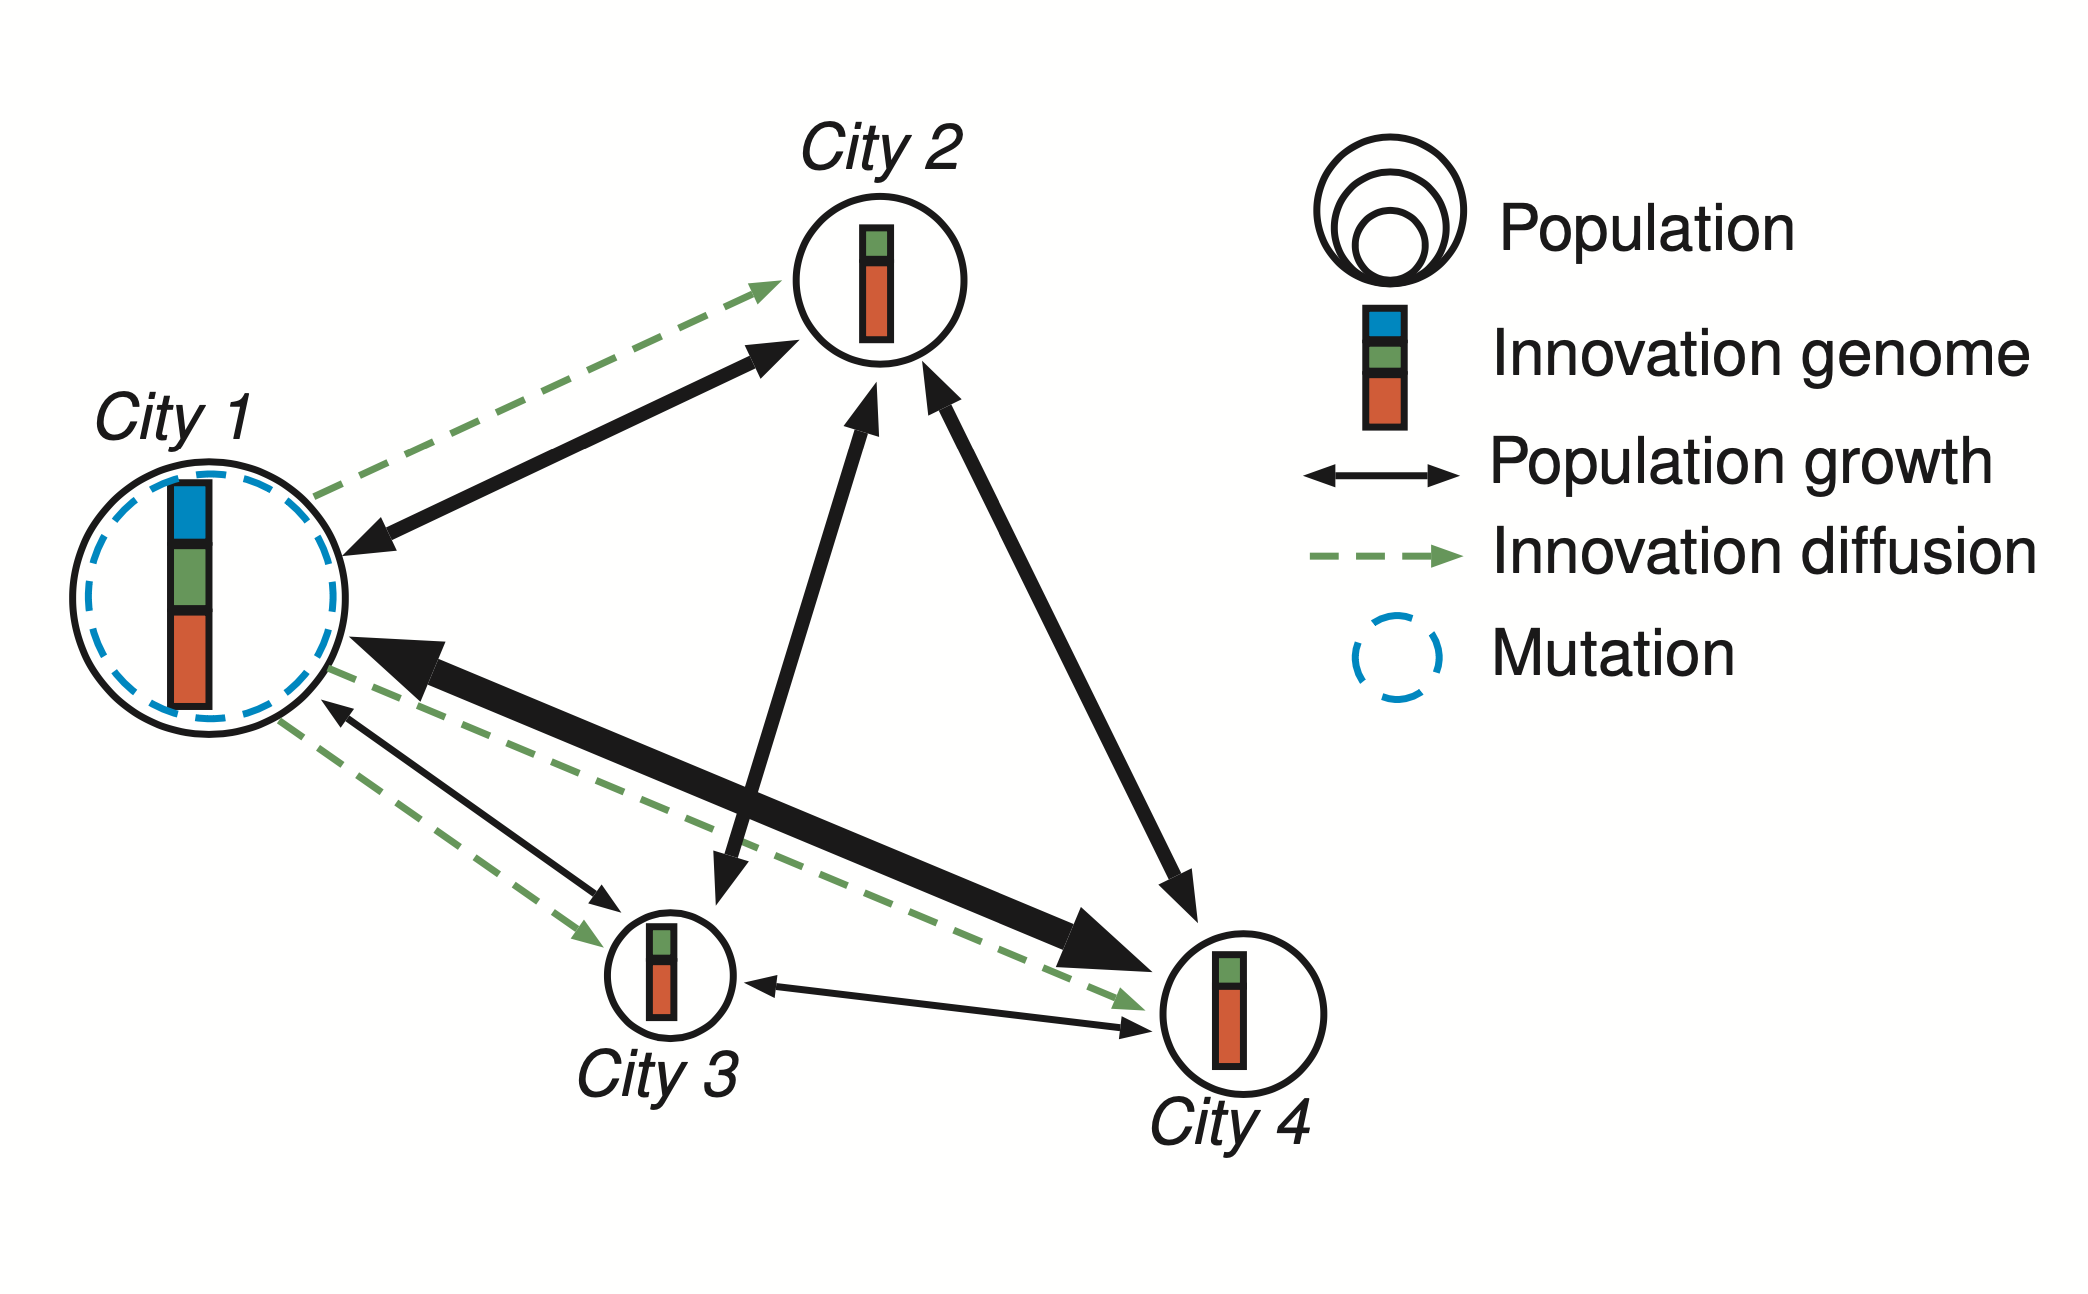
\includegraphics[height=0.4\textheight]{figures/model_4.png}
	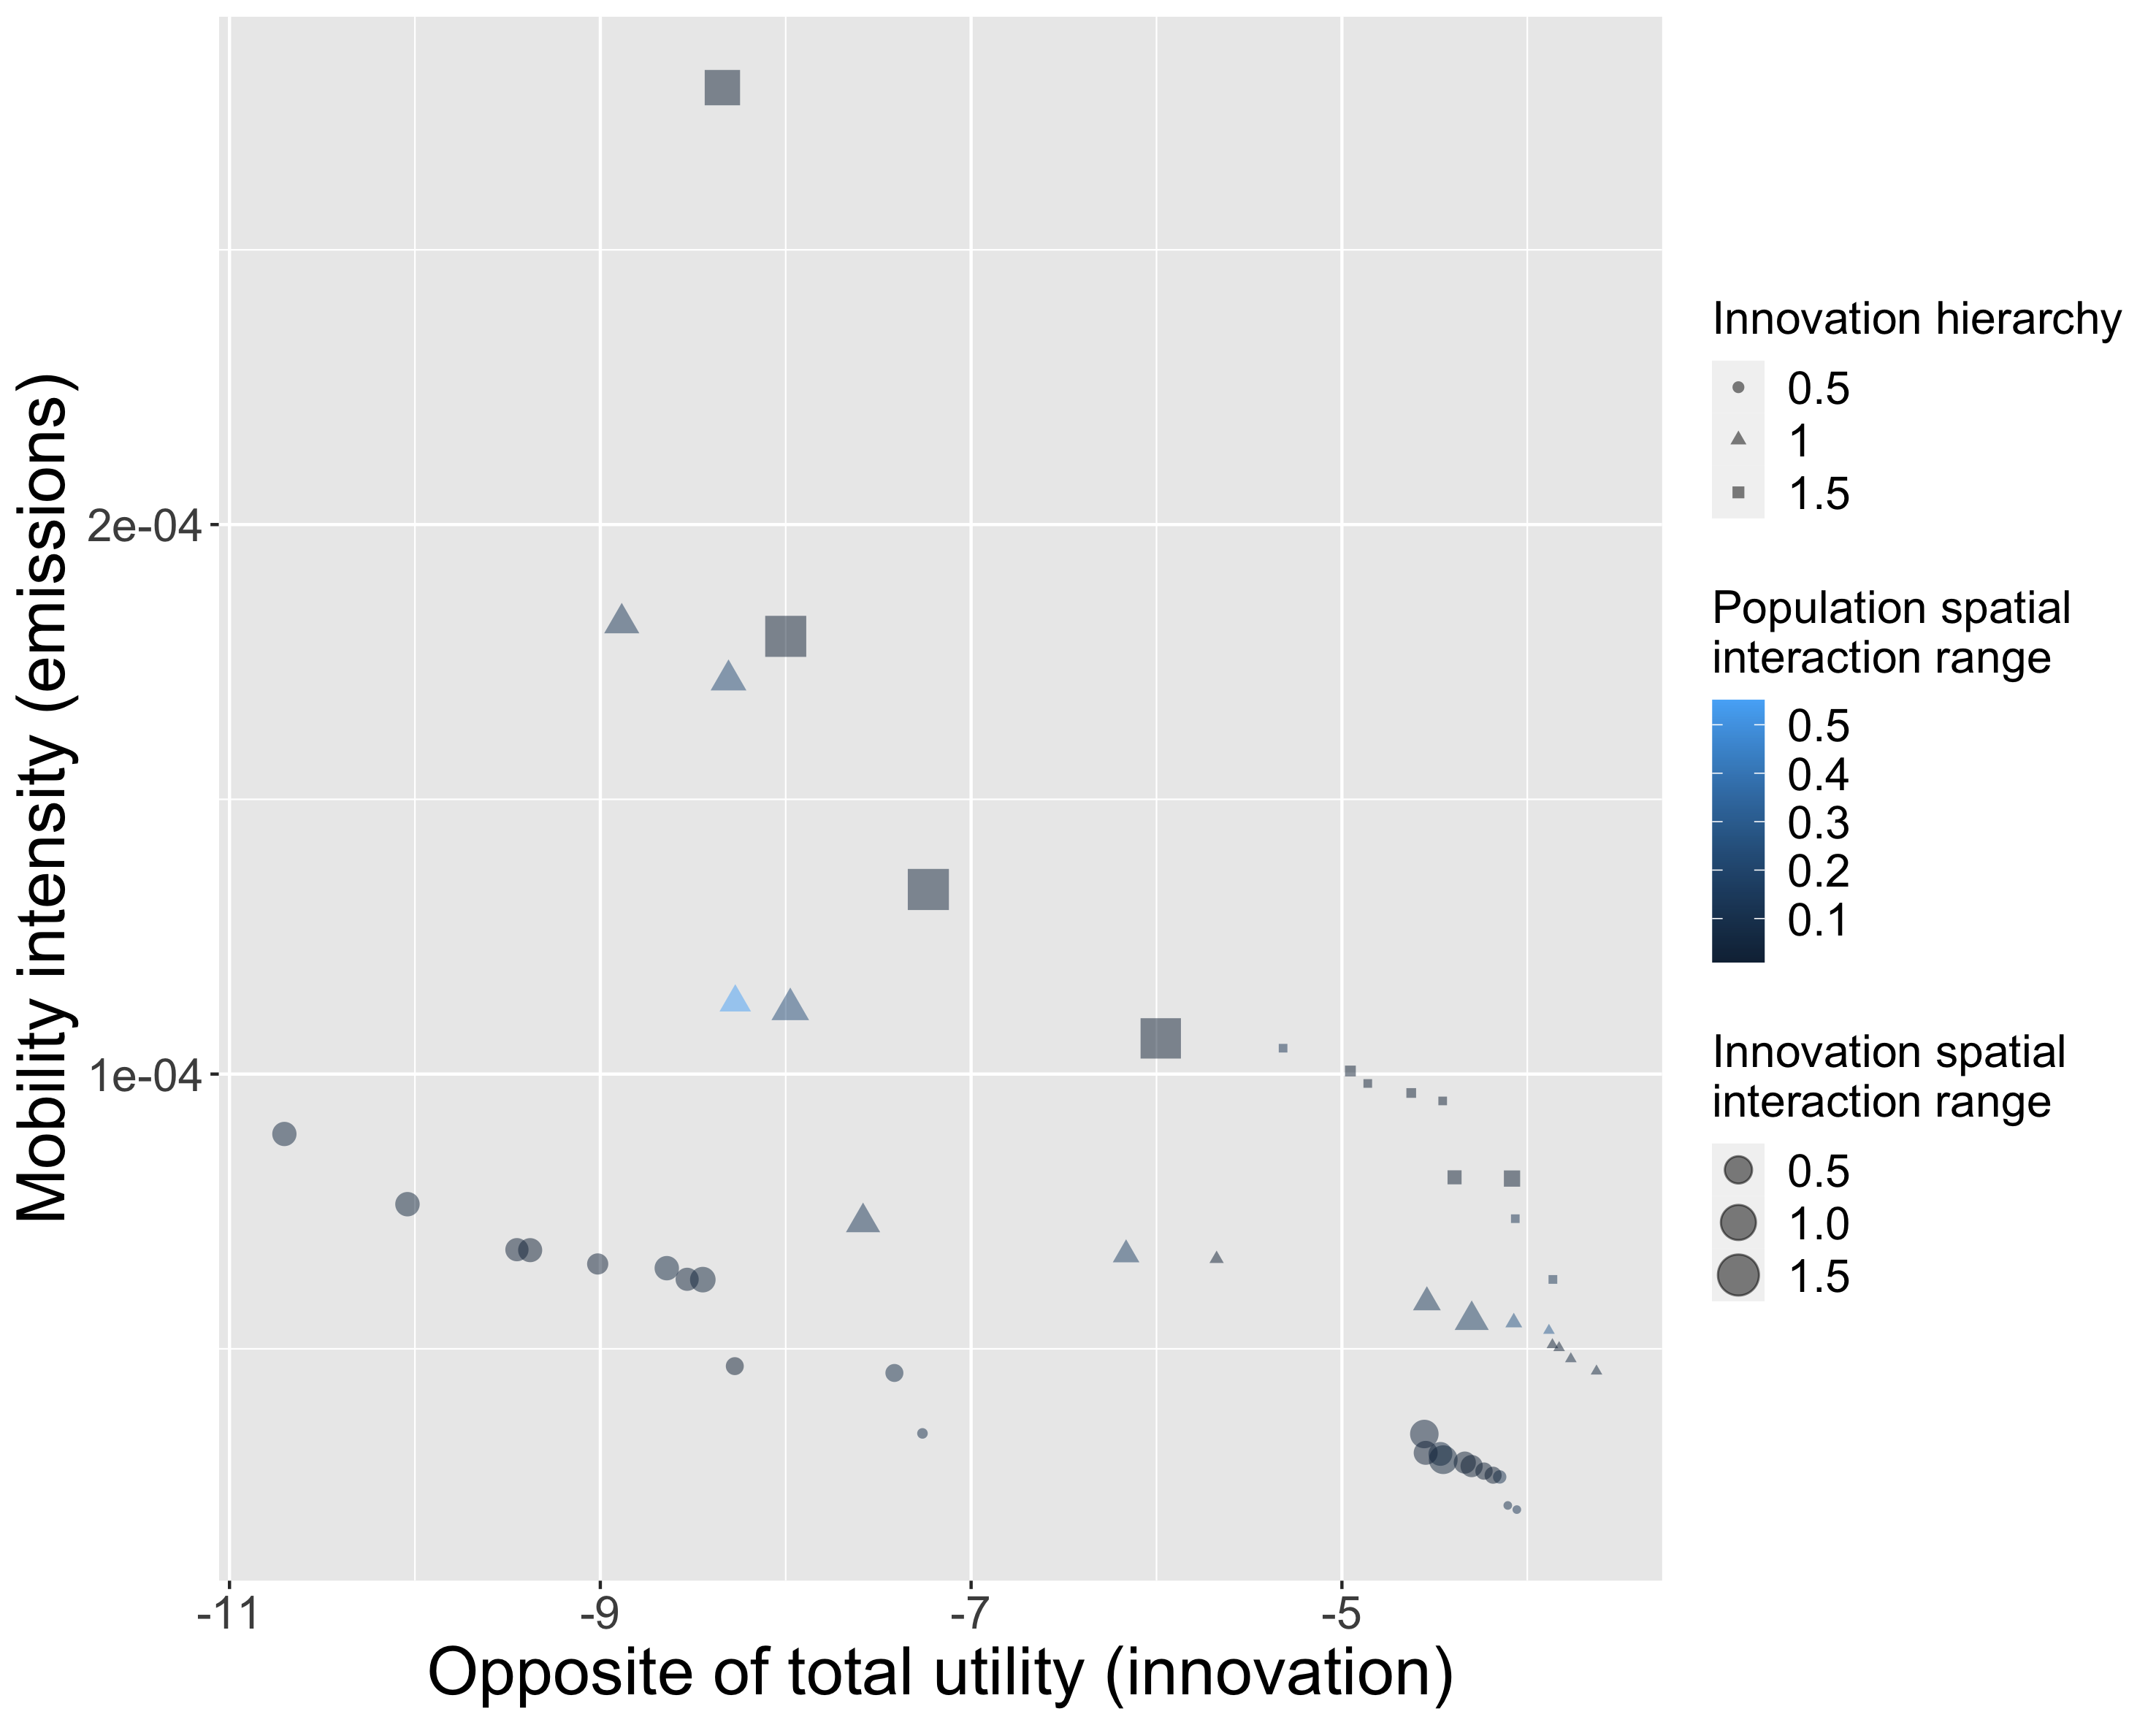
\includegraphics[height=0.4\textheight]{figures/pareto-oppAverageUtility-averageGravityFlow_VARYINGINNOVHIERARCHY_color-gravityDecay_size-innovationDecay.png}
\end{center}


\tiny

Raimbault, J., \& Pumain, D. (2022). Trade-offs between sustainable development goals in systems of cities. Journal of Urban Management.

\nocite{raimbault2022trade}

\bigskip

\normalsize

\textbf{Work in progress: } coupling with an economic exchanges model \cite{cottineau2015modular} and a co-evolution model between transport infrastructure and cities \cite{raimbault2021modeling}

\medskip

$\rightarrow$ many-objective optimisation of proxy indicators for 5 SDGs (emissions, wealth, economic inequalities, innovation, infrastructure).


}




\sframe{Vertical integration: towards multi-scale models}{



\begin{center}
	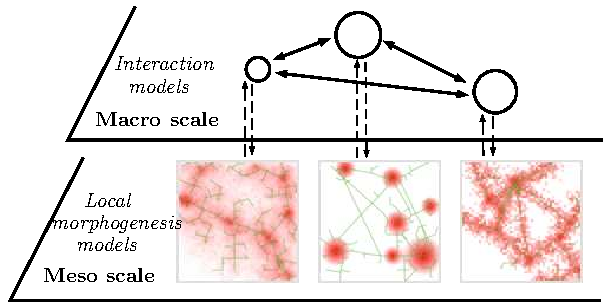
\includegraphics[width=0.75\textwidth]{figures/multiscale_morph.pdf}
\end{center}

\medskip

\textit{Processes specific to scales, coupling implies dedicated ontologies} 

\medskip

\tiny

Raimbault, J. (2021). Strong coupling between scales in a multi-scalar model of urban dynamics. arXiv preprint arXiv:2101.12725.

\nocite{raimbault2021strong}

\smallskip

Raimbault, J. (2021). A multiscale model of urban morphogenesis. arXiv preprint arXiv:2103.17241.

\nocite{raimbault2021multiscale}


}




\sframe{Model exploration methods to foster knowledge integration}{
	
	OpenMOLE software \cite{reuillon2013openmole}: \textit{(i) Innovative exploration methods; (ii) Scaling of methods on high performance computing environments; (iii) Scripts to embed and couple models.}
	
	\smallskip
	
	\centering
	
	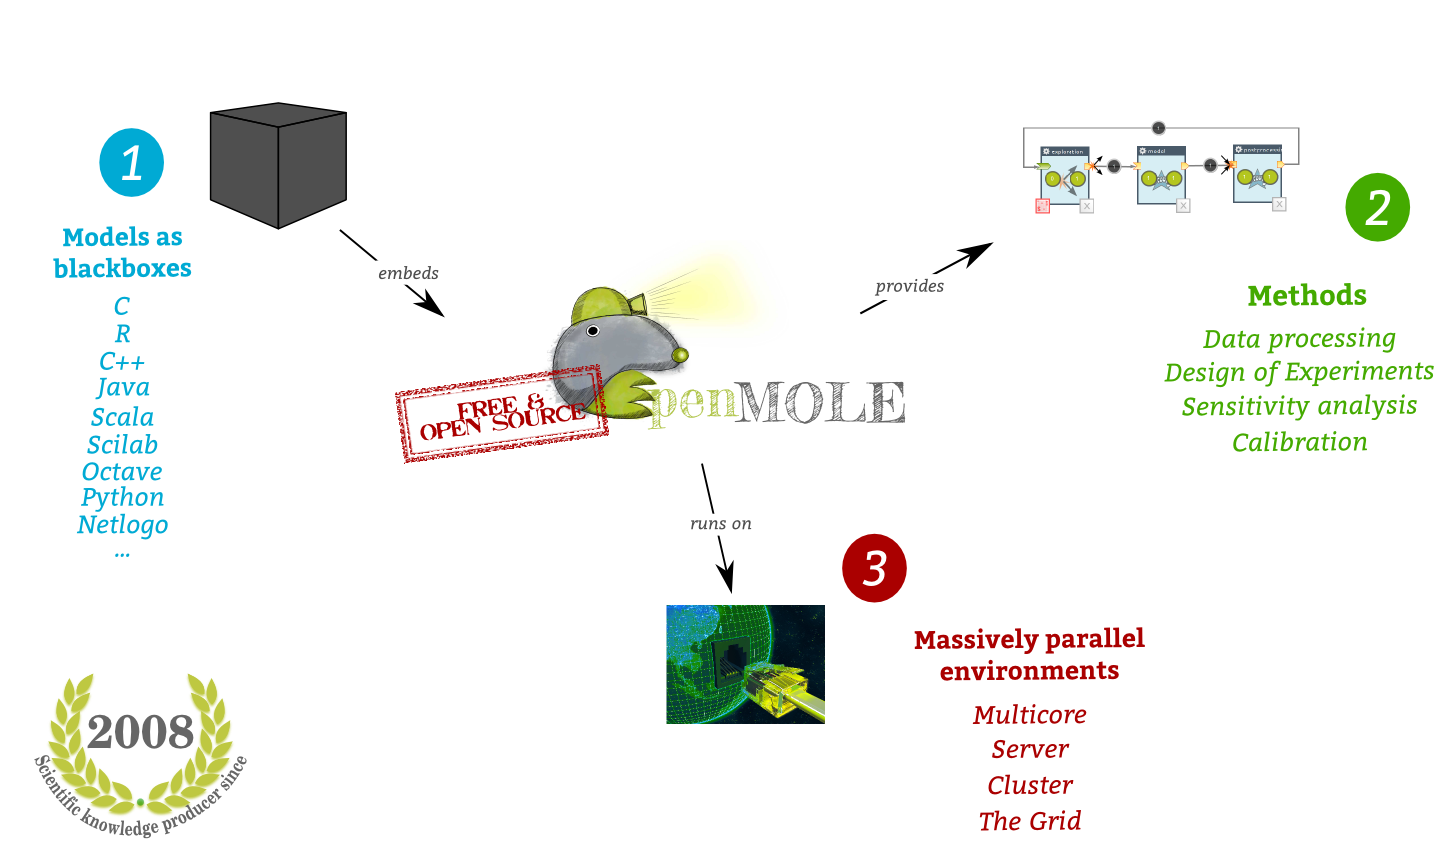
\includegraphics[width=0.8\textwidth]{figures/openmoleGal.png}
	
}




\sframe{Validation: towards spatial sensitivity analysis}{



\centering

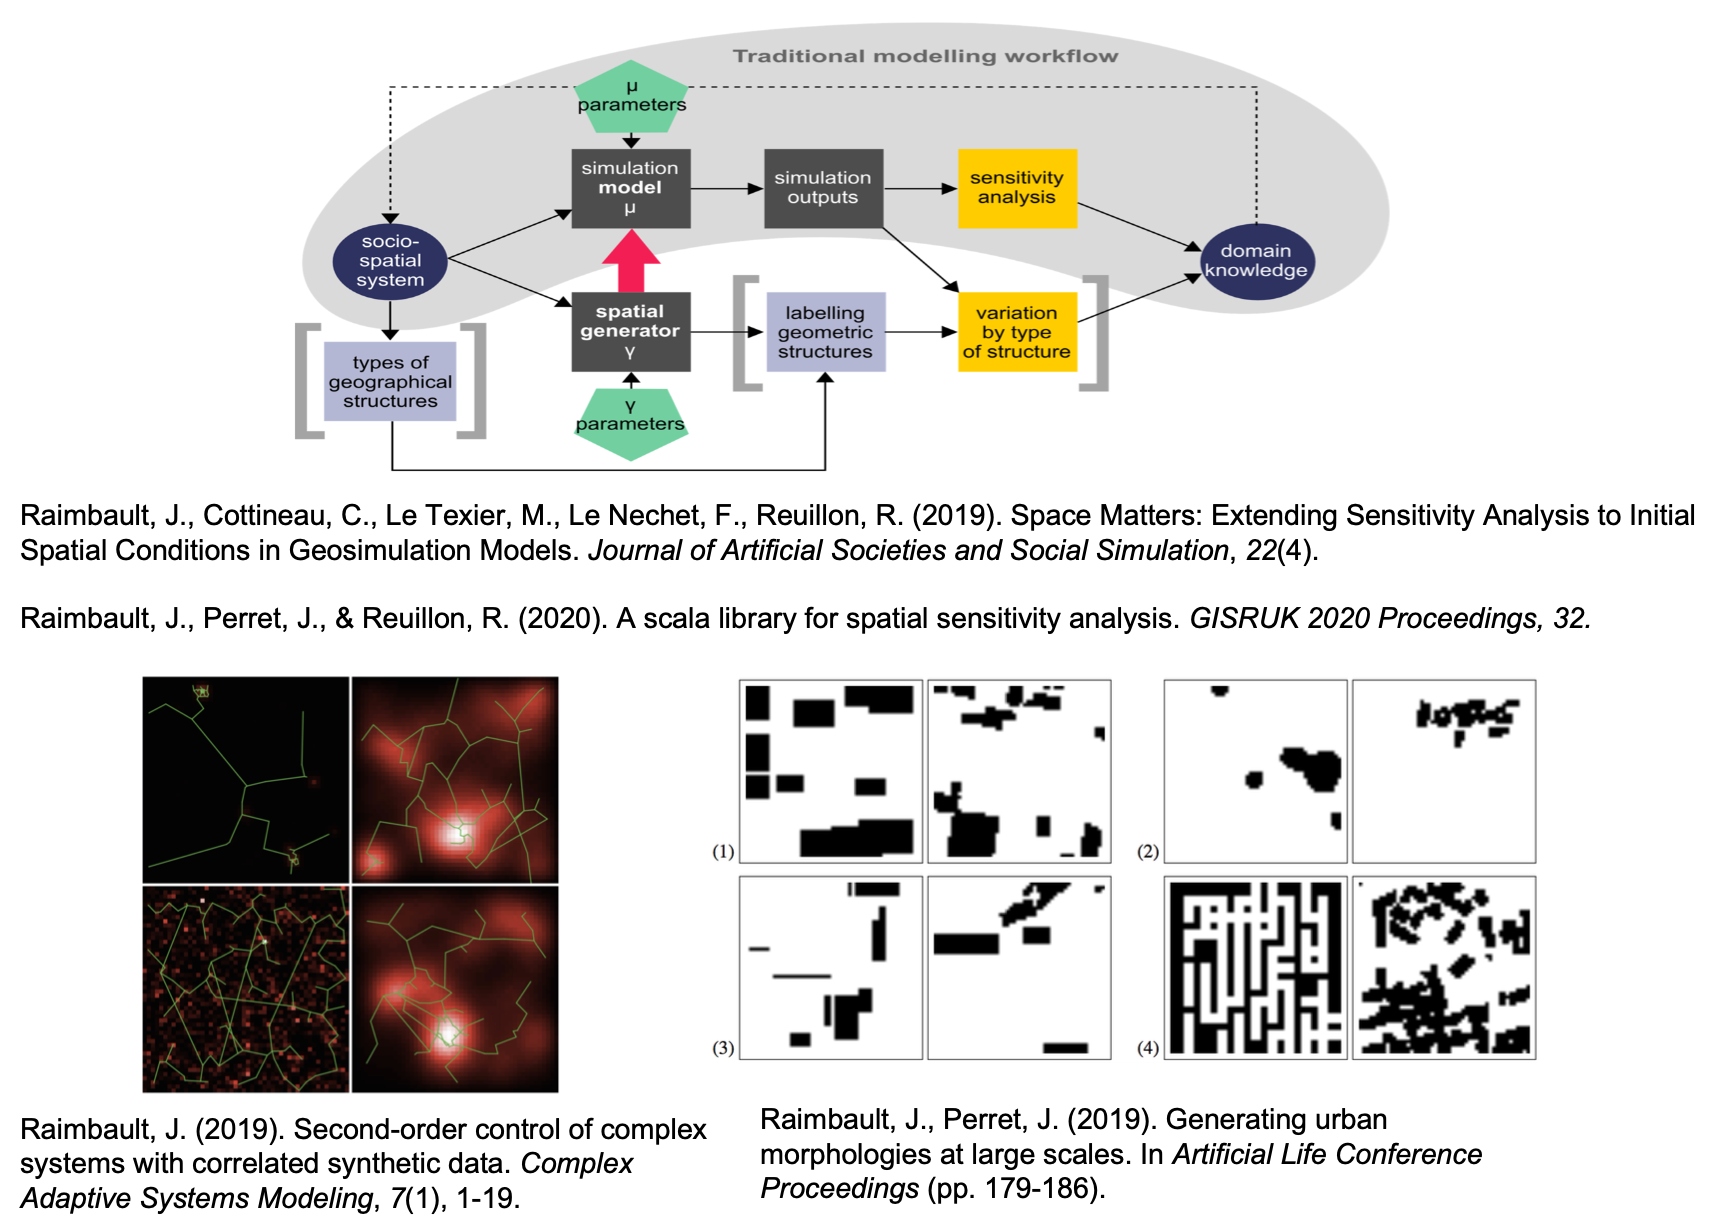
\includegraphics[width=0.95\linewidth]{figures/spatial_sa.png}

\nocite{raimbault2019second}
\nocite{raimbault2019generating}
\nocite{raimbault2019space}

}






\section{Modular open transport models}


\sframe{Sensitivity analysis of MATSim}{

\textit{Large scale urban/transport ABMs must be validated for relevant and robust policy applications}

\bigskip

A few examples of MATSim validation or sensitivity analysis in the literature: uncertainty \cite{bienzeisler2021uncertainty}, sensitivity analysis \cite{zhuge2019sensitivity}, discrete choice parameters \cite{horl2021integrating}


\bigskip
\bigskip

\textbf{Research objective:}

\medskip

\textit{Provide a modular and open implementation of MATSim generic to any UK urban area and test global sensitivity analysis methods on it}

}

\sframe{Land-use transport models}{

\textit{Land-use transport models as a progressive complexification through coupling of detailed sub-models}

\medskip

\begin{center}
	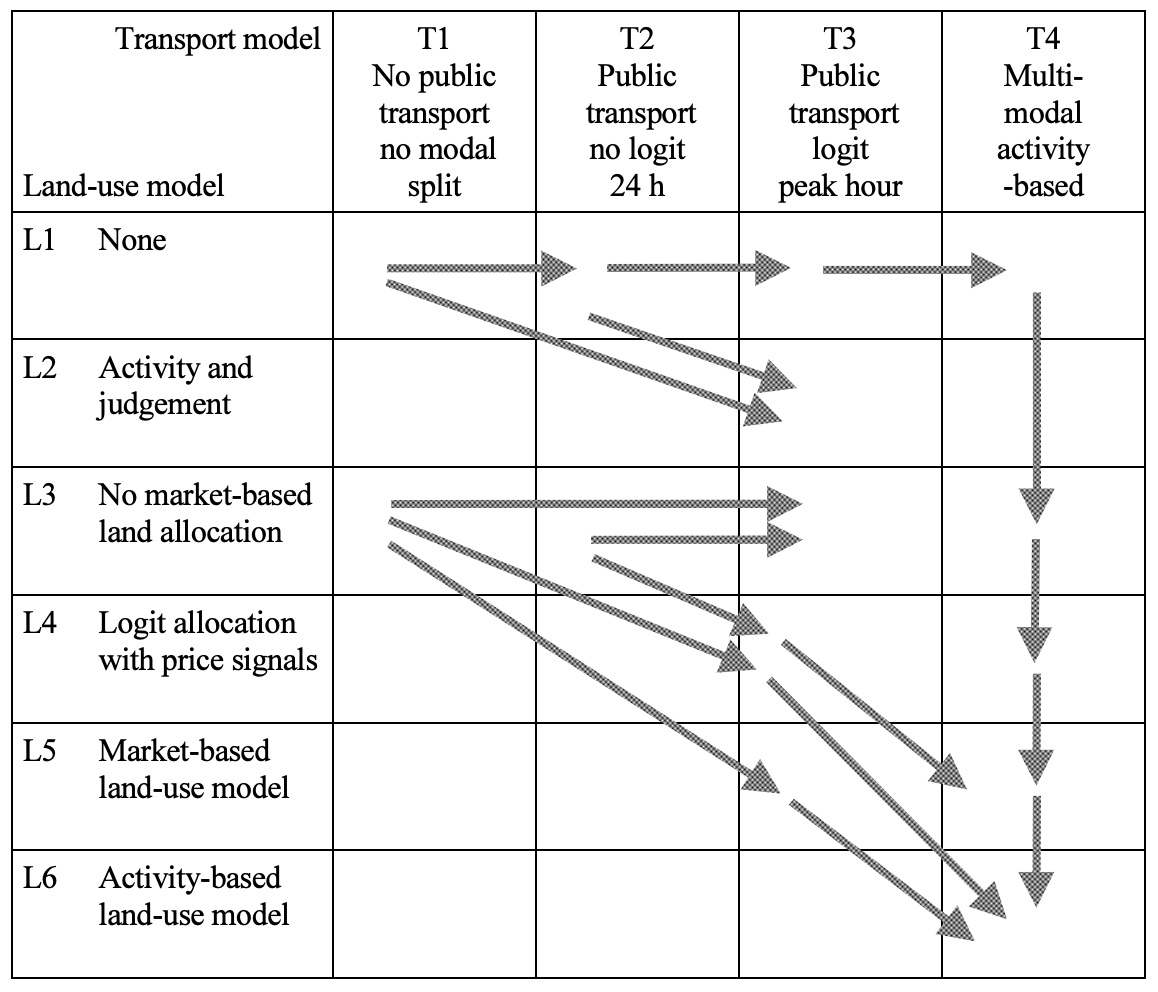
\includegraphics[width=0.45\linewidth]{figures/wegener1.png}\hspace{0.3cm}
	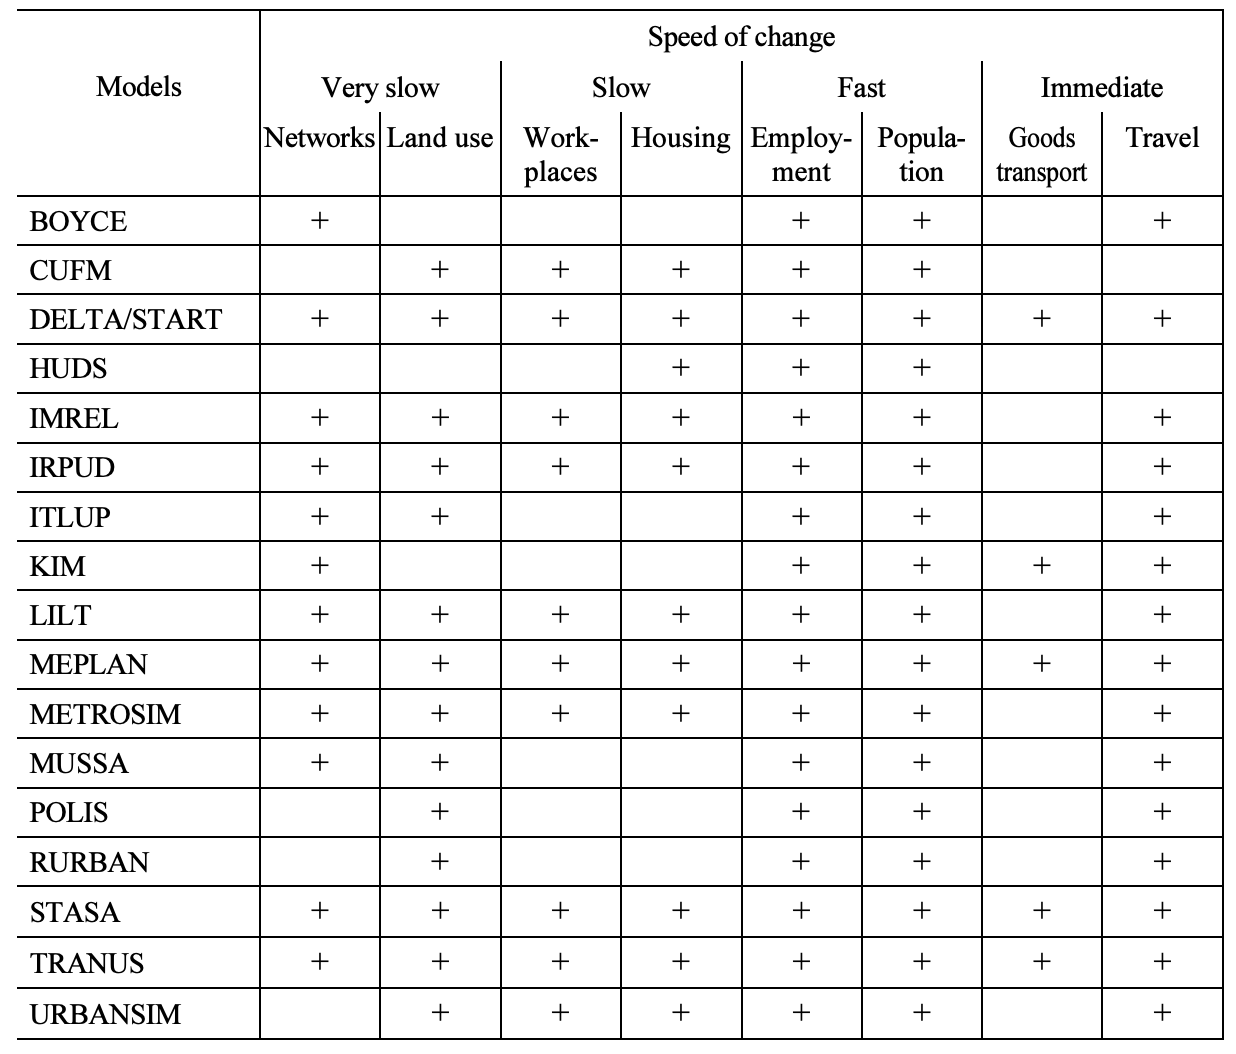
\includegraphics[width=0.45\linewidth]{figures/wegener2.png}
\end{center}

Source: \cite{wegener2004land}

}


\sframe{Urban transportation models}{

\textit{MATSim model: heterogenous data and integration of many sub-models}

\medskip

\begin{center}
	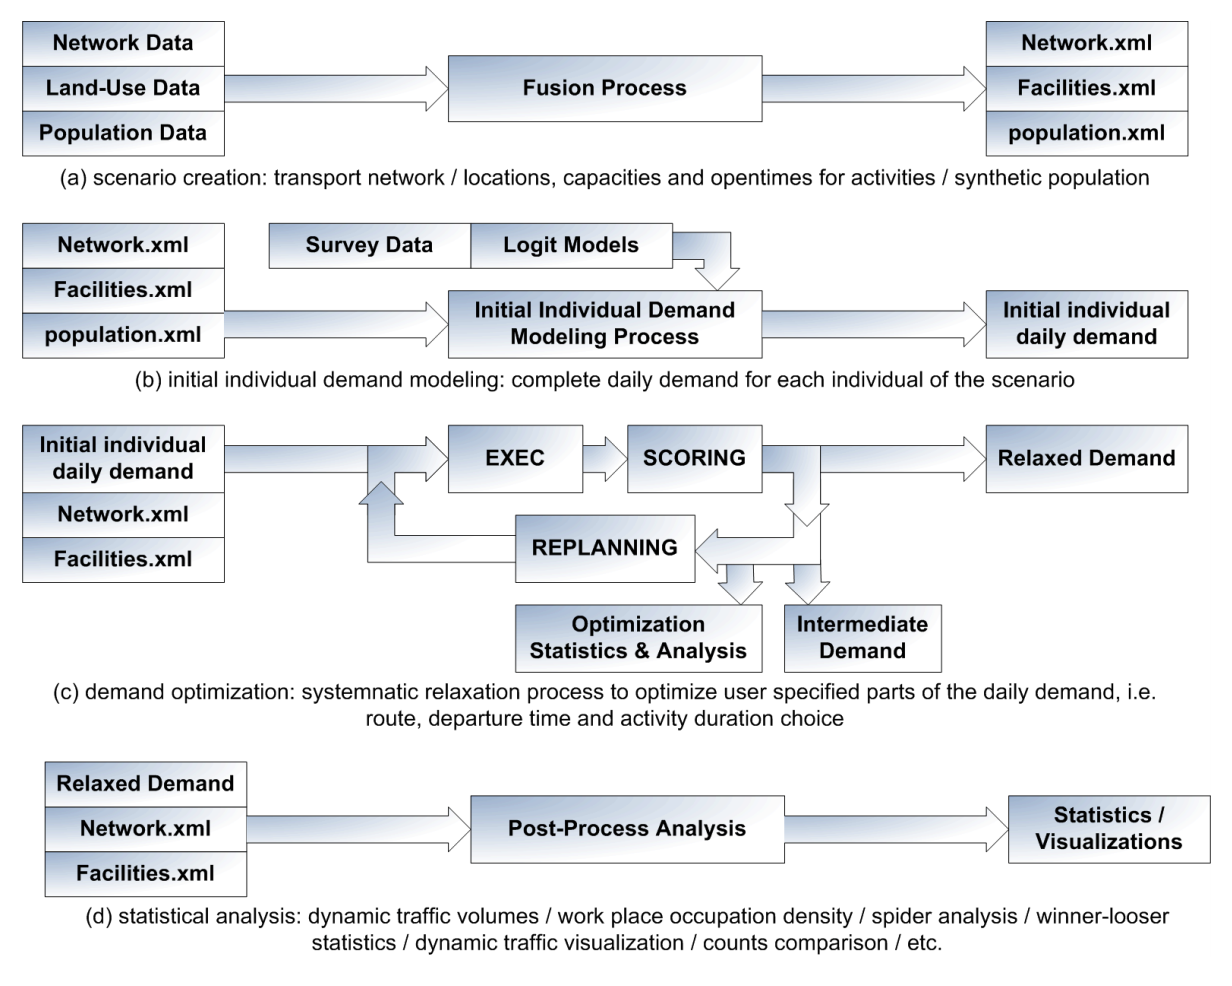
\includegraphics[height=0.7\textheight]{figures/matsim.png}
\end{center}

Source: \cite{balmer2009matsim}

}



\sframe{MATSim model integration}{


\textit{Modular four-step multimodal transportation model using open source projects and data}

\bigskip

\textbf{Integrated models:}

\begin{itemize}
	\item MATSim model (MATSim Community) for the transportation system \url{https://www.matsim.org/} \cite{w2016multi}
	\item SPENSER model (University of Leeds) for the synthetic population \url{https://github.com/nismod/microsimulation} \cite{spooner2021dynamic}
	\item QUANT model (CASA, University College London) for spatial interactions to generate home-work plans \url{http://quant.casa.ucl.ac.uk/} \cite{batty2021new} 
	\item spatialdata library (OpenMOLE community) for data processing \url{https://github.com/openmole/spatialdata} \cite{raimbault2020scala}
\end{itemize}

\smallskip

\tiny

Raimbault, J., \& Batty, M. (2021). Estimating public transport congestion in UK urban areas with open transport models. GISRUK 2021 Proceedings.

\nocite{raimbault2021estimating}

}




\sframe{Data and implementation}{

\footnotesize


\textbf{Data:} Generic for any Functional Urban Area (GHSL \cite{florczyk2019ghsl}) or any arbitrary area in the UK: NOMIS census, OrdnanceSurvey roads, Traveline National Dataset for public transport

\medskip

\textbf{Workflow system for the integration of submodels and validation experiments:}
 OpenMOLE software \url{https://openmole.org/} \cite{reuillon2013openmole}


\medskip

\textbf{Implementation}

\begin{itemize}
	\item Synthetic SPENSER population distributed at the micro level using OSM buildings
	\item QUANT model to generate home-work commuting flows, job locations determined by sampling flows
	\item Network and plans (simple uniform commuting plans) prepared into MATSim xml files and fed into a multimodal MATSim model
	\item Models integrated as Docker containers
\end{itemize}

\medskip

\textbf{Open source: } docker files to build model containers and integration script available at\\
\texttt{https://github.com/JusteRaimbault/UrbanDynamics/tree/master/Models/Matsim}

}

\sframe{Data preparation}{

$\rightarrow$ Road network preprocessing: implemented into the \texttt{spatialdata} scala library \cite{raimbault2020scala}

\begin{center}
	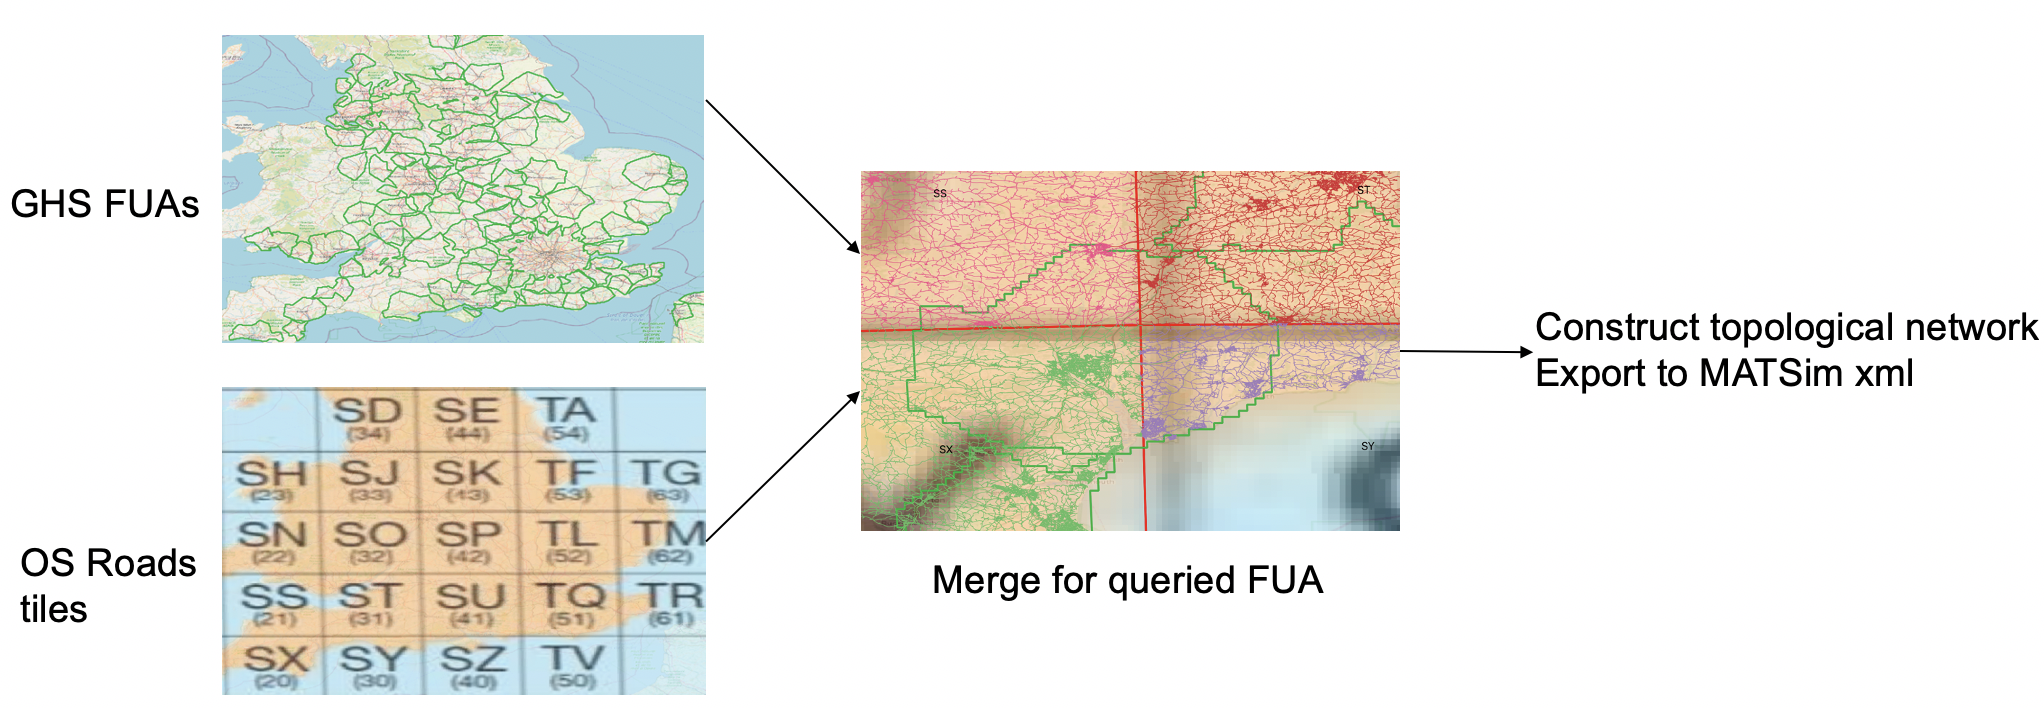
\includegraphics[width=\textwidth]{figures/road_data.png}
\end{center}

\bigskip

$\rightarrow$ Public transport data: from TransXchange (TNDS) to GTFS using UK2GTFS R package \cite{UK2GTFS}; GTFS to MATSim xml schedule using \texttt{pt2matsim} library



}


\sframe{Explored parameters}{

\textit{Parameter sampled for the sensitivity analysis:}

\begin{itemize}
	\item Functional Urban Area (spatial context \cite{raimbault2019space})
	\item Random seed (influence of stochasticity \cite{bienzeisler2021uncertainty})
	\item Synthetic population sampling
	\item Modal choice parameters \cite{horl2021integrating}: mode constants in scoring function (car, public transport, walking)
\end{itemize}


}

\sframe{OpenMOLE script}{

\centering

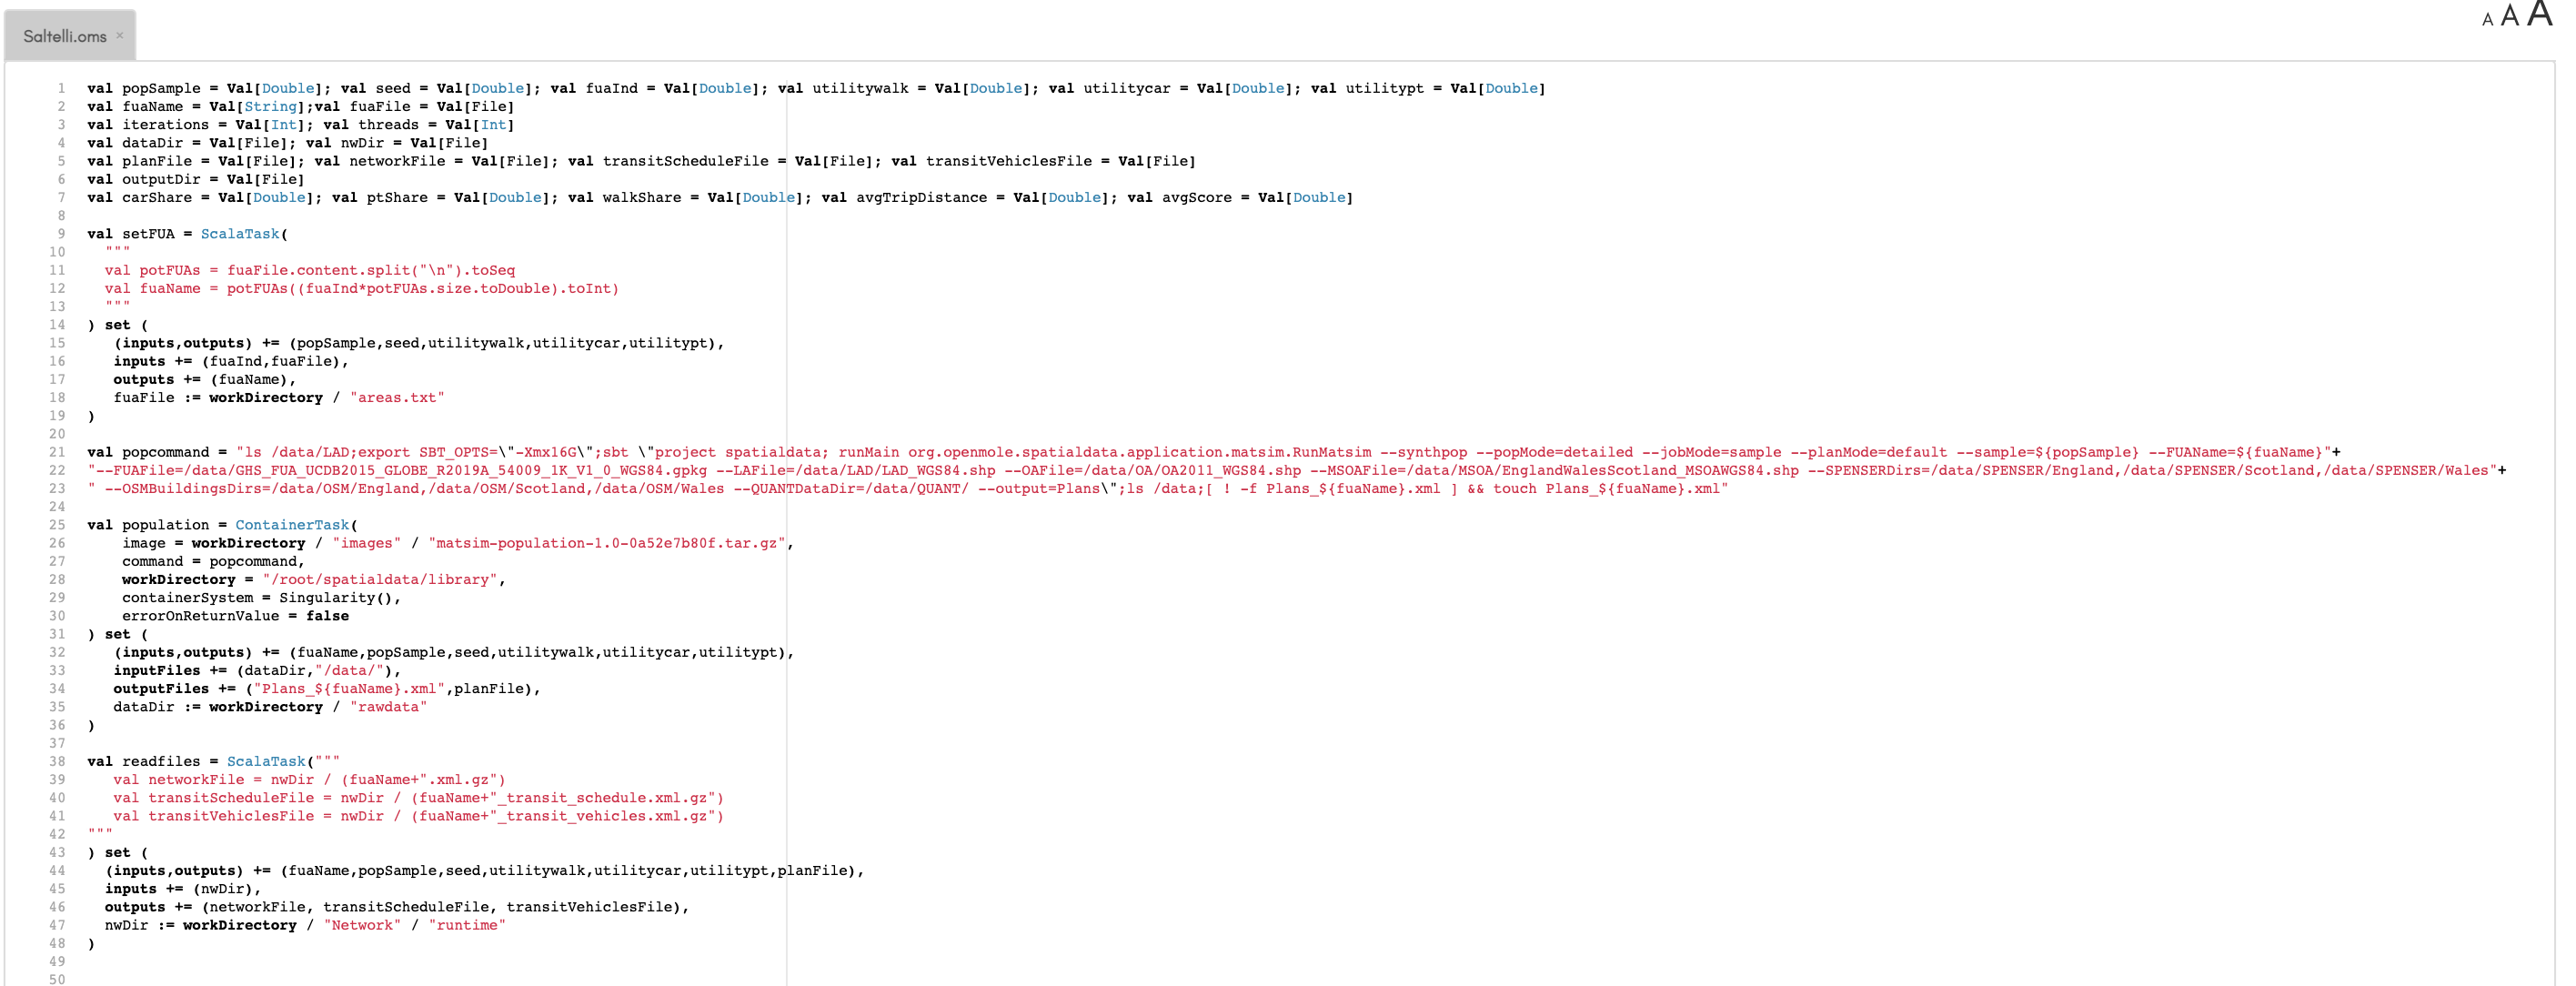
\includegraphics[width=1.1\linewidth]{figures/script_1.png}


}

\sframe{OpenMOLE script (continued)}{


\centering

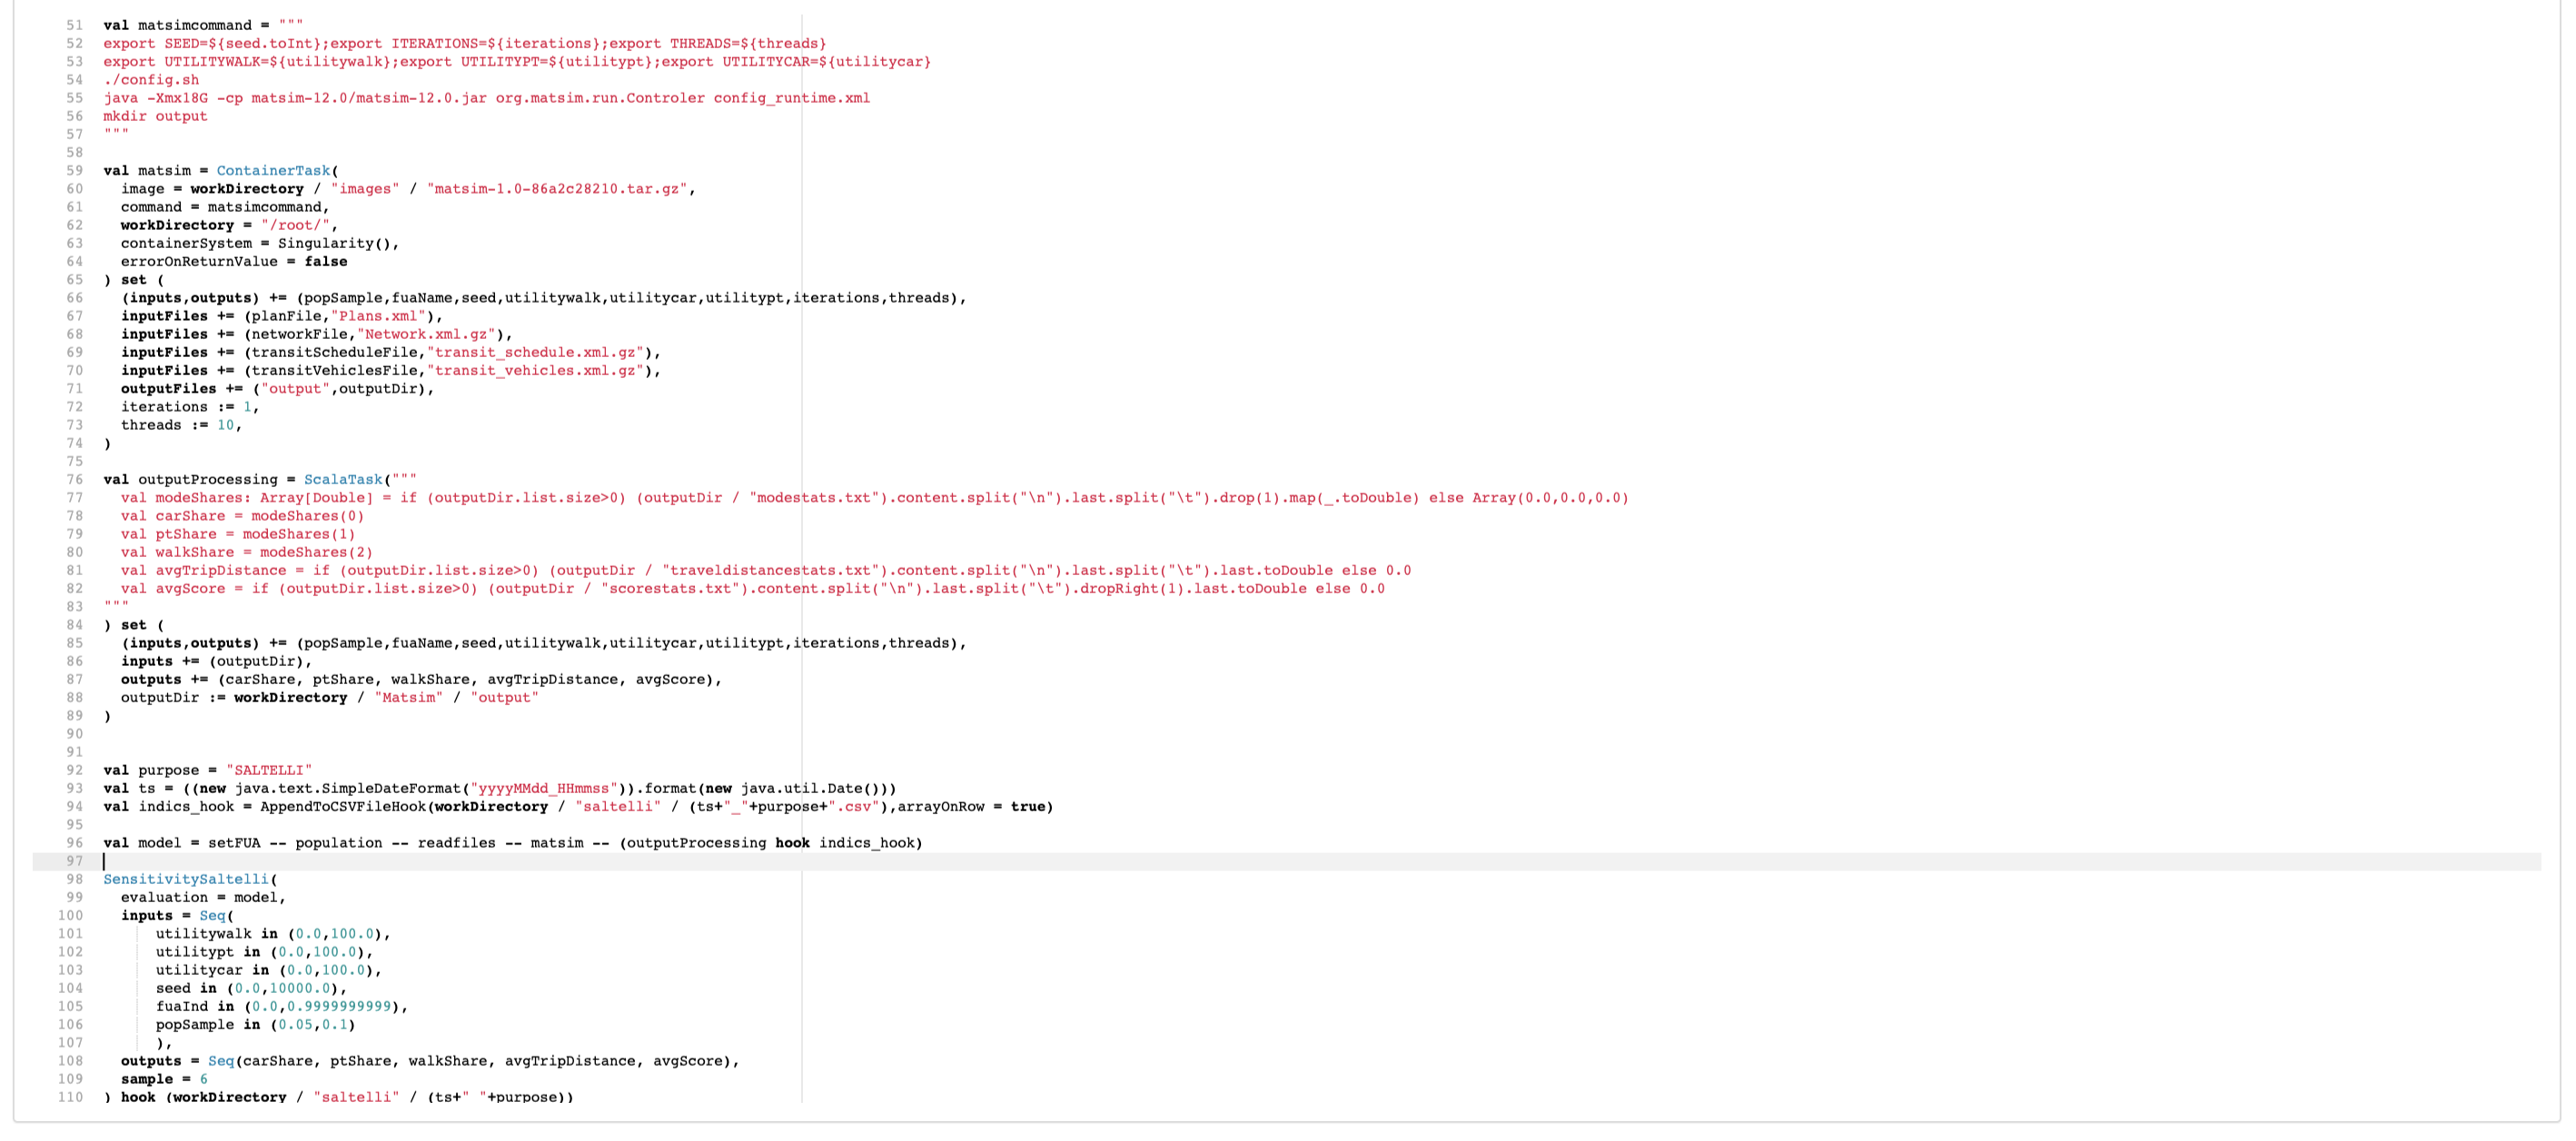
\includegraphics[width=1.1\linewidth]{figures/script_2.png}

}

\sframe{Role of stochasticity}{

\begin{center}
	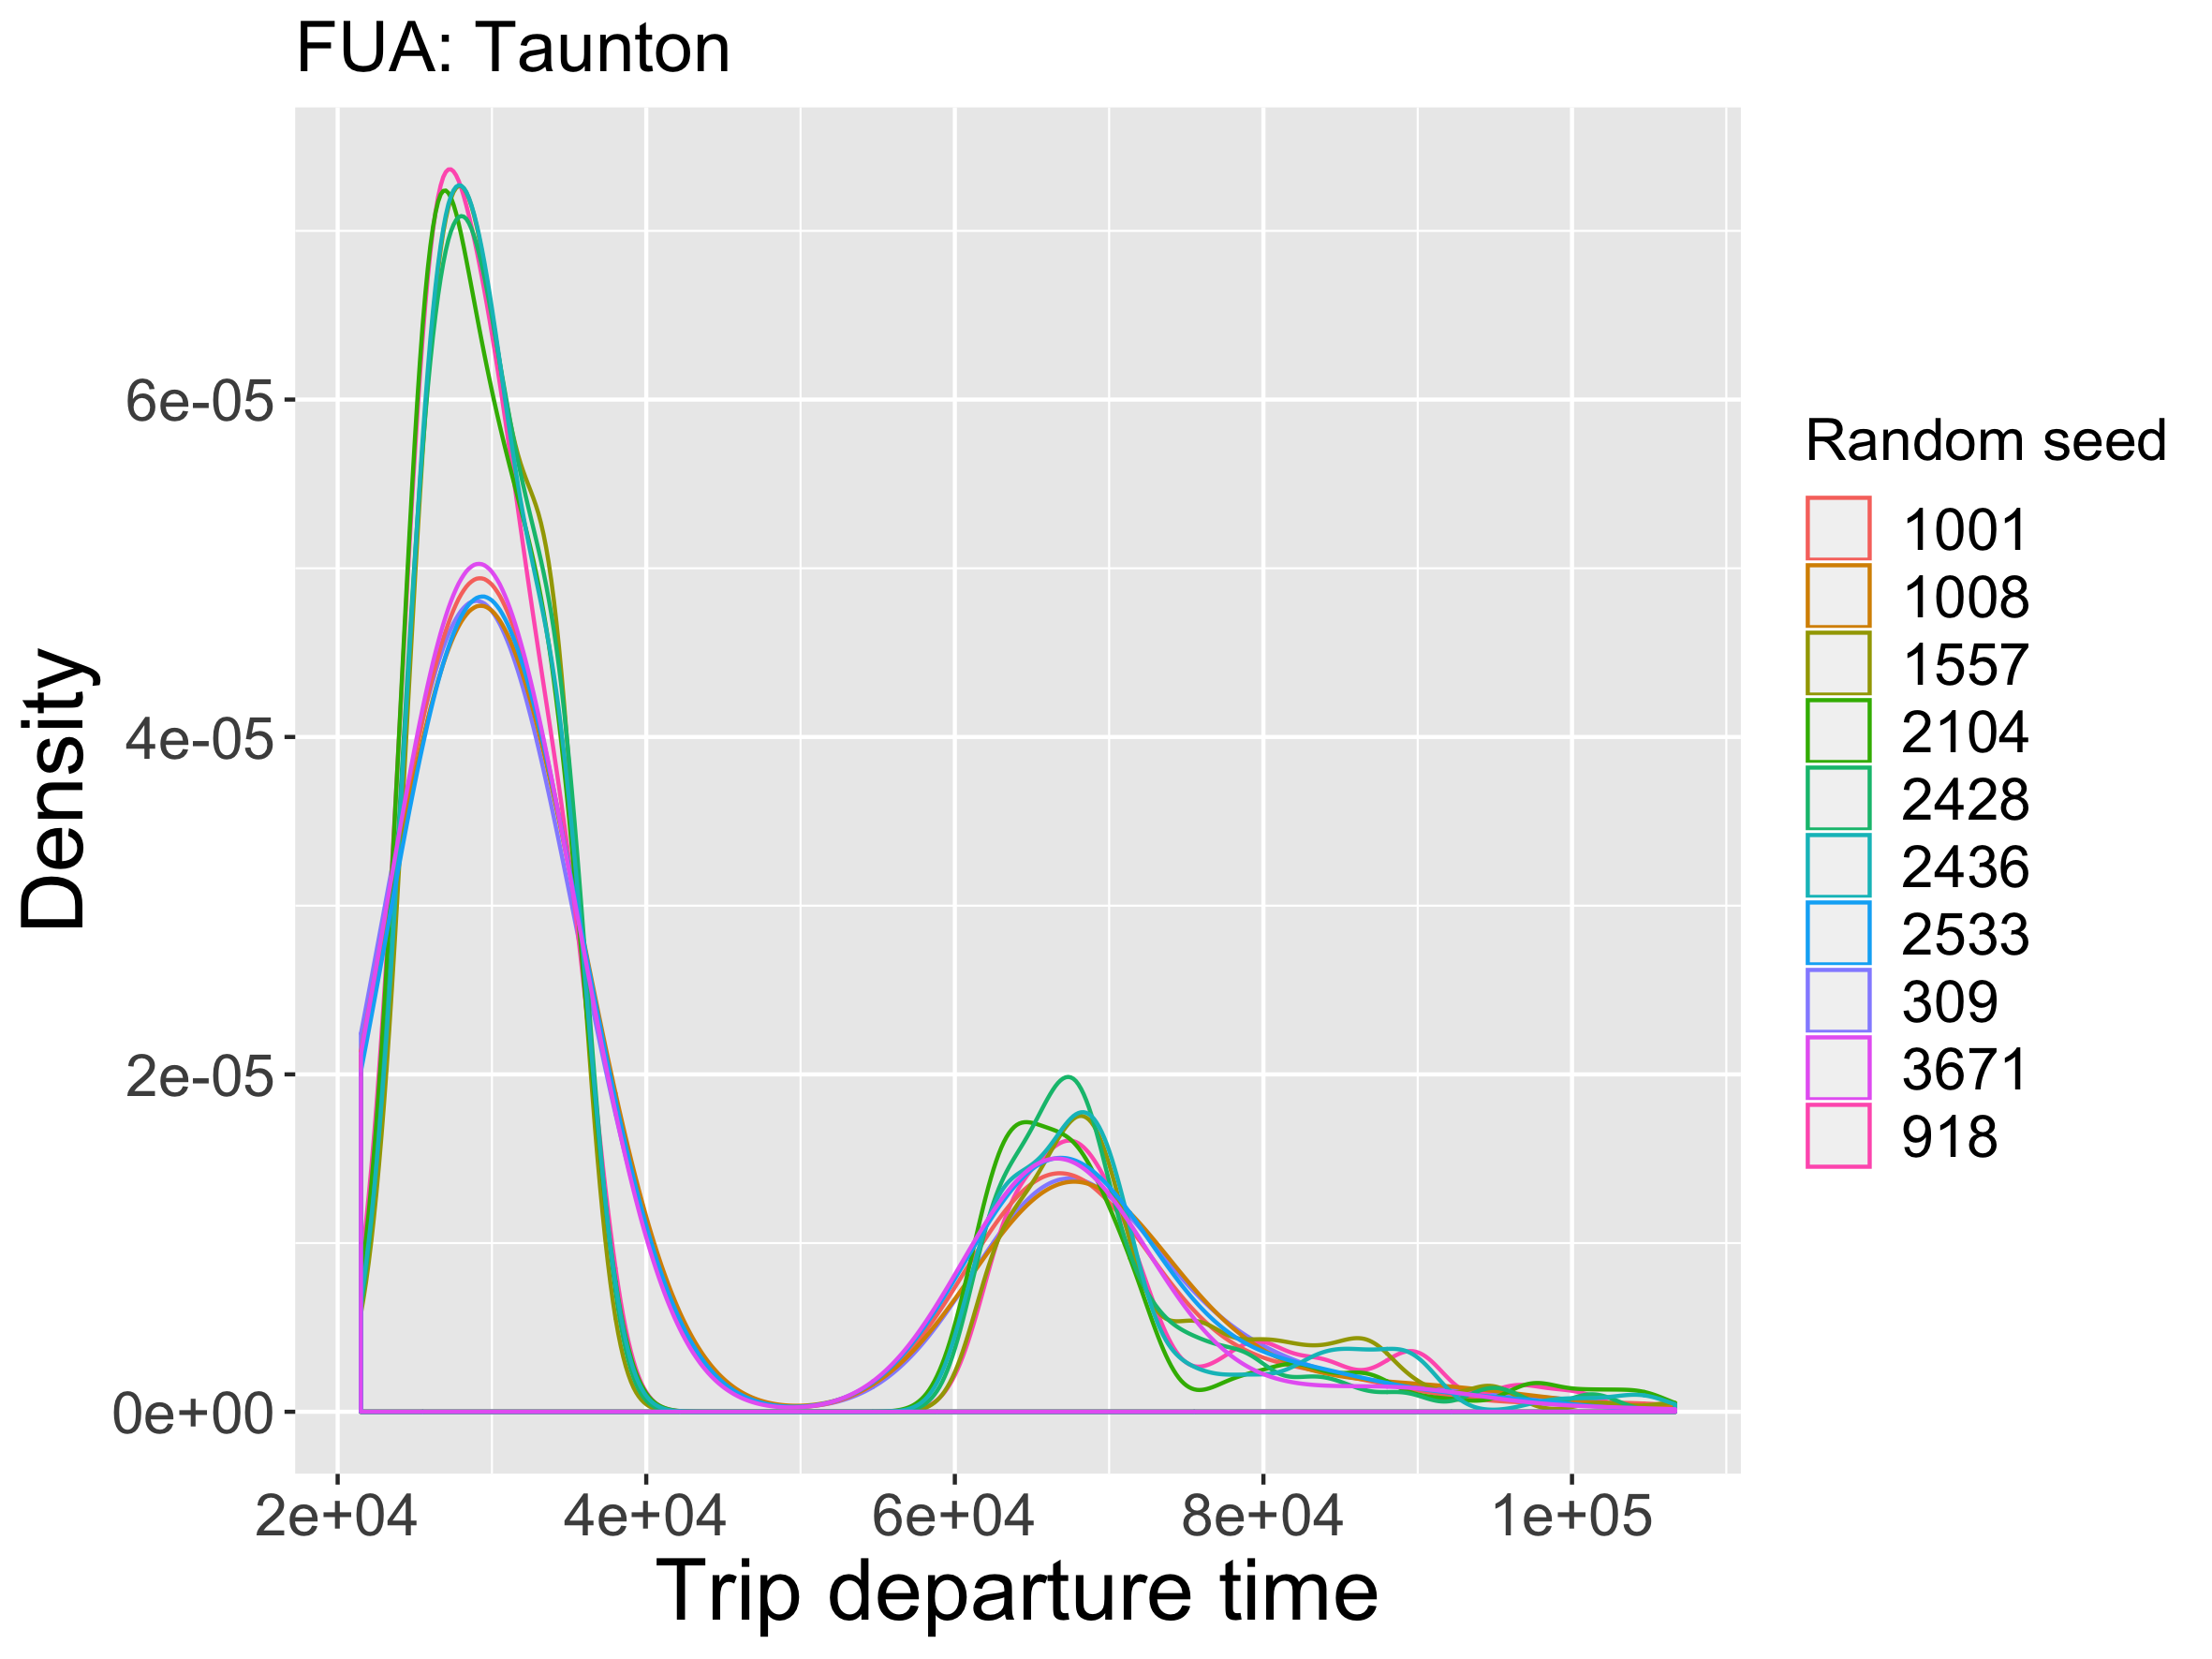
\includegraphics[width=0.9\linewidth]{figures/stochasticity_Taunton.png}
\end{center}


}


\sframe{Global Sensitivity Analysis}{


\textit{Method based on the estimation of conditional relative variances}

\cite{saltelli2010variance}

\medskip

\textbf{First order index}

\[
S_i \textrm{=} \frac{Var \left[ E_{\mathbf{X}_{\sim i}} \left(Y | X_i \right) \right]}{Var\left[Y\right]}
\]

is the expected relative variance reduction if $X_i$ would be fixed

\medskip

\textbf{Total effect index}
\[
ST_i \textrm{=} \frac{E_{\mathbf{X}_{\sim i}}\left[Var\left(Y | \mathbf{X}_{\sim i}\right) \right]}{Var\left[Y\right]}
\]

is the expected relative variance if all factors but $X_i$ are fixed (includes interaction effects)



}


\sframe{GSA results}{


\begin{center}
\begin{tabular}{|c|c|c|c|c|c|c|}
	\hline
	output & $\beta_W$ & $\beta_{PT}$ & $\beta_{C}$ & S & FUA & $p$ \\\hline
carShare & 0.023 & 0.0058 & 0.0079 & 3.94  & 0.165 & 0.379 \\
ptShare & 0.0081 & 0.0074 & 0.0030 & 2.164 & 0.04 & 0.0169 \\
walkShare & 0.0059 & 0.0017 & 0.0074 & 0.834 & 0.16 & 0.082 \\
avgTripDistance & 0.11 & 0.19 & 0.087 & 0.04 & 1.51 & 0.049 \\
avgScore & 0.43 & 0.0003 & 0.0039 & 0.057 & 0.0085 & 0.0073 \\\hline
\end{tabular}
\end{center}

\medskip

\textit{Total order Saltelli indices obtained with $\simeq 50$ model runs}

}






\section{Anticipating the impact of future transportation infrastructure}

\sframe{Coupling QUANT and SPENSER models}{

}

\sframe{Current work and prospects}{

% open questions with spenser-quant coupling

}



\section{Discussion}


\sframe{Discussion}{

% discussion

% Matsimm

% Still a long way to go: a lot of tuning even with containers; issue of infrastructure (memory vs CPUs)

% Some models are intrinsically interactive/visual (cf QUANT): compatible with workflow systems / integration? (change in model function)

% dynamical strong coupling of models (SPENSER/QUANT); applications to policies

% Varenne - mmodel functions - couling/integrqtion / issues different

% DEF and characterisation of model coupling: horizontal/vertical ; strength of coupling -> URGENT do some work (SR/MetaAnal) - rassembler idees - paper as primer?



}



\sframe{Conclusion}{

$\rightarrow$ \textbf{Integrated models} capturing complexity of \textbf{urban sustainability} towards \textbf{decision-making}.

\medskip

$\rightarrow$ \textbf{Robust} knowledge from models obtained with the development of \textbf{validation and exploration methods}.


\medskip

$\rightarrow$ \textbf{Complementarity} of perspectives, models and theories in an \textbf{interdisciplinary} context.

%\medskip

%$\rightarrow$ Which kind of interdisciplinarity?
% as a comment only: building bridges, while deep knowledge in each discipline? ~


\bigskip
\bigskip
\bigskip

\textbf{To use OpenMOLE (free and open software) and contribute: }\\
\url{https://openmole.org}

\bigskip

\textbf{Presented models open source at }

\url{https://github.com/JusteRaimbault/UrbanDynamics}

}









%%%%%%%%%%%%%%%%%%%%%
\begin{frame}[allowframebreaks]
\frametitle{References}
\bibliographystyle{apalike}
\bibliography{biblio}
\end{frame}
%%%%%%%%%%%%%%%%%%%%%%%%%%%%





\end{document}




